\documentclass[aspectratio=169,11pt,hyperref={colorlinks=true}]{beamer}
\usetheme{boxes}
\setbeamertemplate{navigation symbols}{}
\definecolor{openstack}{RGB}{149,0,4}
\setbeamercolor{titlelike}{fg=openstack}
\setbeamercolor{structure}{fg=openstack}
\hypersetup{colorlinks,urlcolor=openstack}
\setbeamertemplate{footline}[frame number]
% Inserting graphics
\usepackage{graphicx}
% Side-by-side figures, etc
\usepackage{subfigure}
% Code snippits
\usepackage{listings}

\usepackage{lmodern}
% Color stuff
\usepackage{color}
\usepackage{amsmath}
\usepackage{amssymb}
\usepackage{empheq}
\usepackage[braket, qm]{qcircuit}
\usepackage{tikz}
\usepackage{gensymb}
\newcommand\RBox[1]{%
  \tikz\node[draw,rounded corners,align=center,] {#1};%
}
\usepackage{hyperref}
%\usecolortheme{buzz}
%\usecolortheme{wolverine}
%\usetheme{Boadilla}
\usepackage[T1]{fontenc}

\definecolor{mygreen}{rgb}{0,0.6,0}
\definecolor{mygray}{rgb}{0.5,0.5,0.5}
\definecolor{mymauve}{rgb}{0.58,0,0.82}

\lstset{%
  backgroundcolor=\color{white},   % choose the background color; you must add \usepackage{color} or \usepackage{xcolor}
  breakatwhitespace=false,         % sets if automatic breaks should only happen at whitespace
  breaklines=true,                 % sets automatic line breaking
  captionpos=b,                    % sets the caption-position to bottom
  commentstyle=\color{openstack},  % comment style
  extendedchars=true,              % lets you use non-ASCII characters; for 8-bits encodings only, does not work with UTF-8
  keepspaces=true,                 % keeps spaces in text, useful for keeping indentation of code (possibly needs columns=flexible)
  keywordstyle=\color{blue},       % keyword style
%  otherkeywords={*,...},           % if you want to add more keywords to the set
  numbersep=5pt,                   % how far the line-numbers are from the code
  numberstyle=\tiny\color{mygray}, % the style that is used for the line-numbers
  rulecolor=\color{black},         % if not set, the frame-color may be changed on line-breaks within not-black text (e.g. comments (green here))
  showspaces=false,                % show spaces everywhere adding particular underscores; it overrides 'showstringspaces'
  showstringspaces=false,          % underline spaces within strings only
  showtabs=false,                  % show tabs within strings adding particular underscores
  stringstyle=\color{openstack},   % string literal style
}


\setbeamerfont{caption}{series=\normalfont,size=\fontsize{6}{8}}
\setbeamertemplate{caption}{\raggedright\insertcaption\par}

\setlength{\abovecaptionskip}{0pt}
\setlength{\floatsep}{0pt}

\author[Matthew Treinish]{%
    \texorpdfstring{%
        \centering
        Matthew Treinish\\
        Software Engineer - IBM Research\\
        \href{mailto:mtreinish@kortar.org}{mtreinish@kortar.org}\\
        \texttt{mtreinish on Freenode}\\
        \href{https://github.com/mtreinish/open-source-quantum-computing}{https://github.com/mtreinish/open-source-quantum-computing}
   }
   {Matthew Treinish}
}
\date{January 25, 2019}

\title{Open Source Quantum Computing}
\begin{document}

\titlepage

\section{What is a Quantum Computer}
\begin{frame}
    % All my cryptos broke
\end{frame}

\newcommand{\iu}{{i\mkern1mu}}

\begin{frame}
    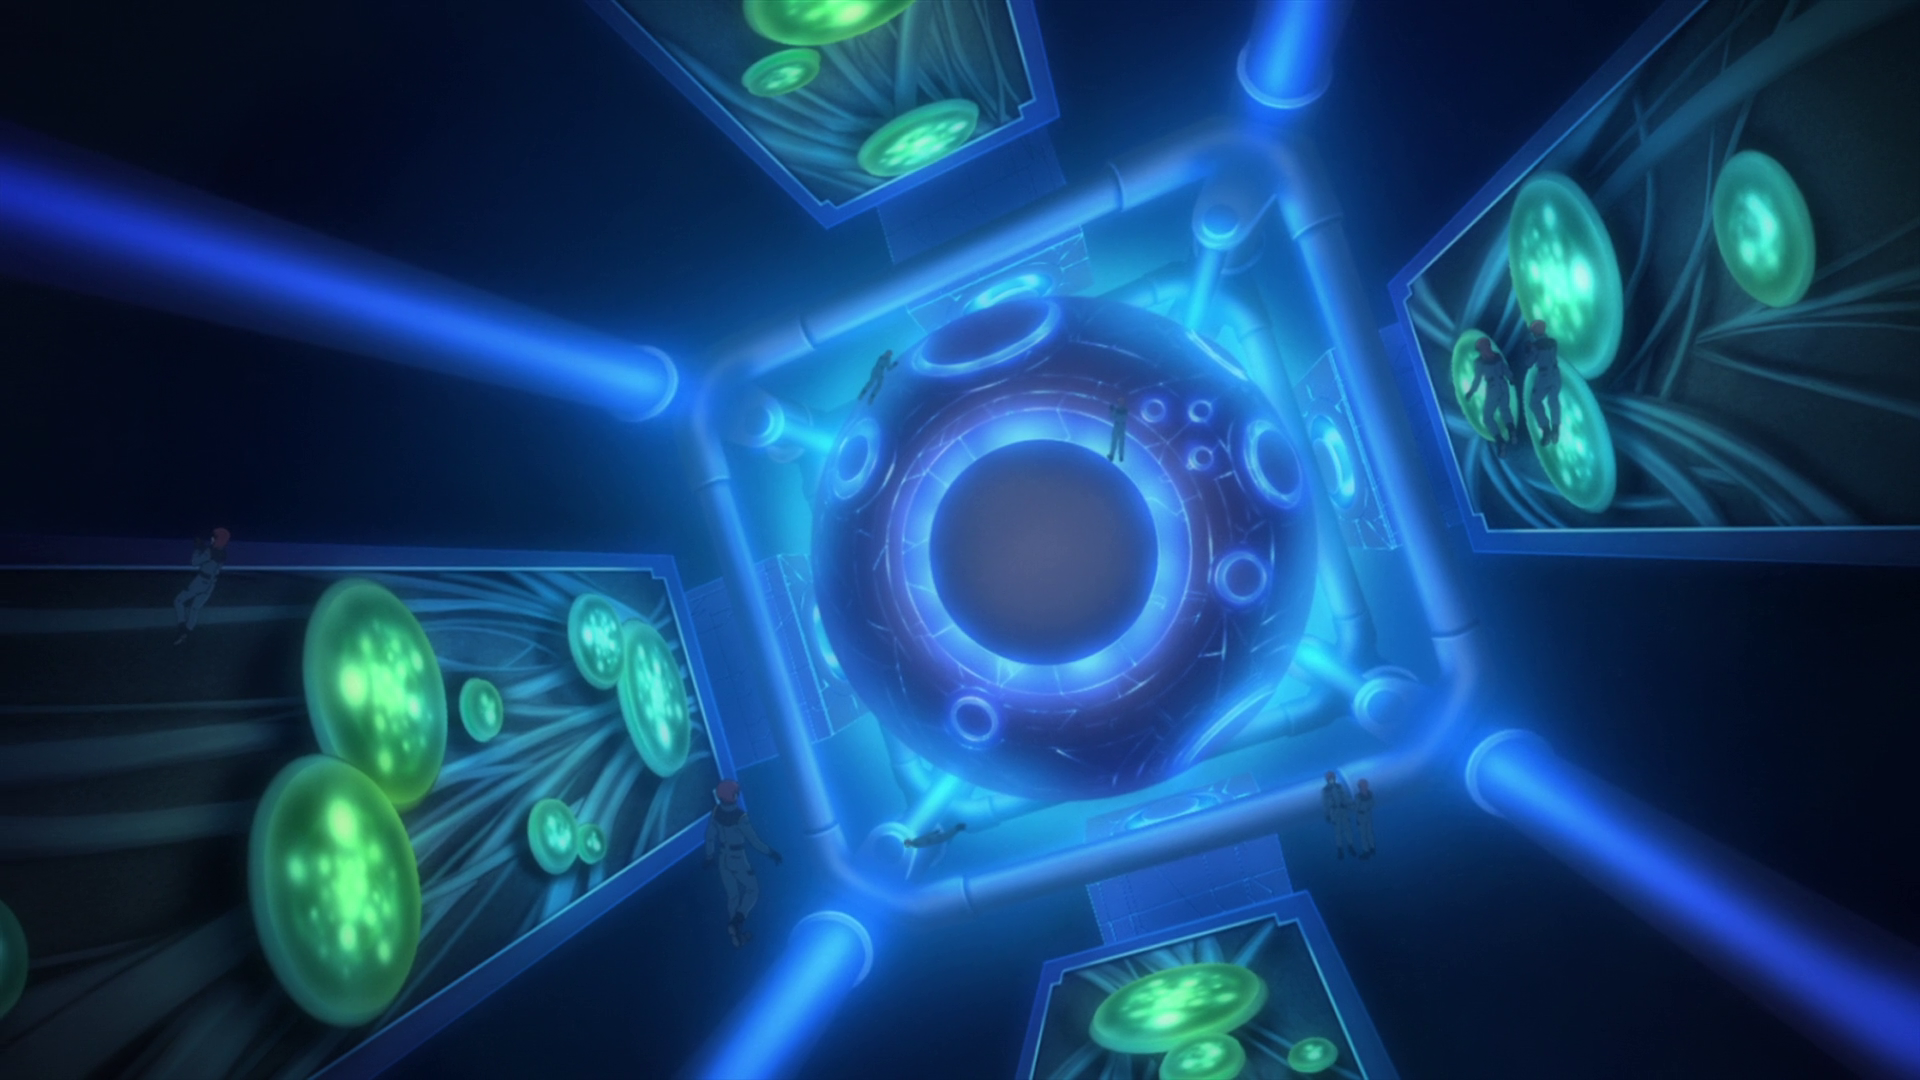
\includegraphics[width=\textwidth]{Veda_AD2314.png}
\end{frame}

\begin{frame}
    \frametitle{Real Quantum Computer}
    \begin{columns}[t]
        \column{.5\textwidth}
            \centering
            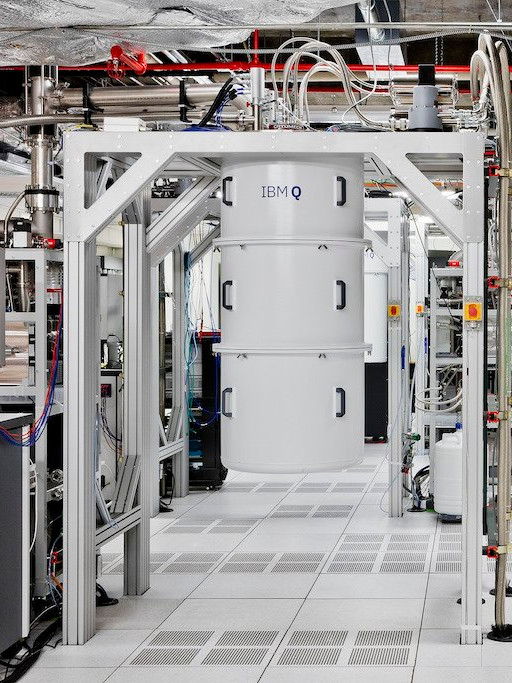
\includegraphics[height=.45\textheight]{outside.jpg}\\
            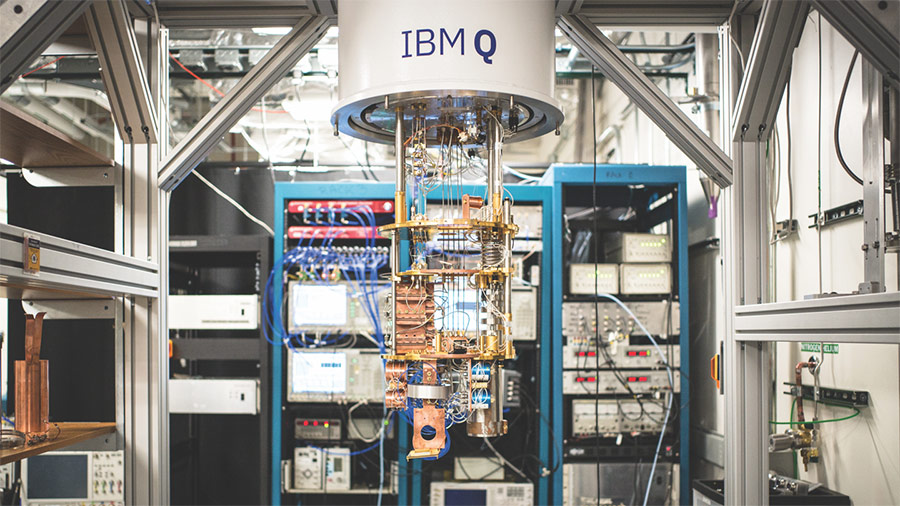
\includegraphics[height=.45\textheight]{inside-1.jpg}
        \column{.5\textwidth}
            \centering
            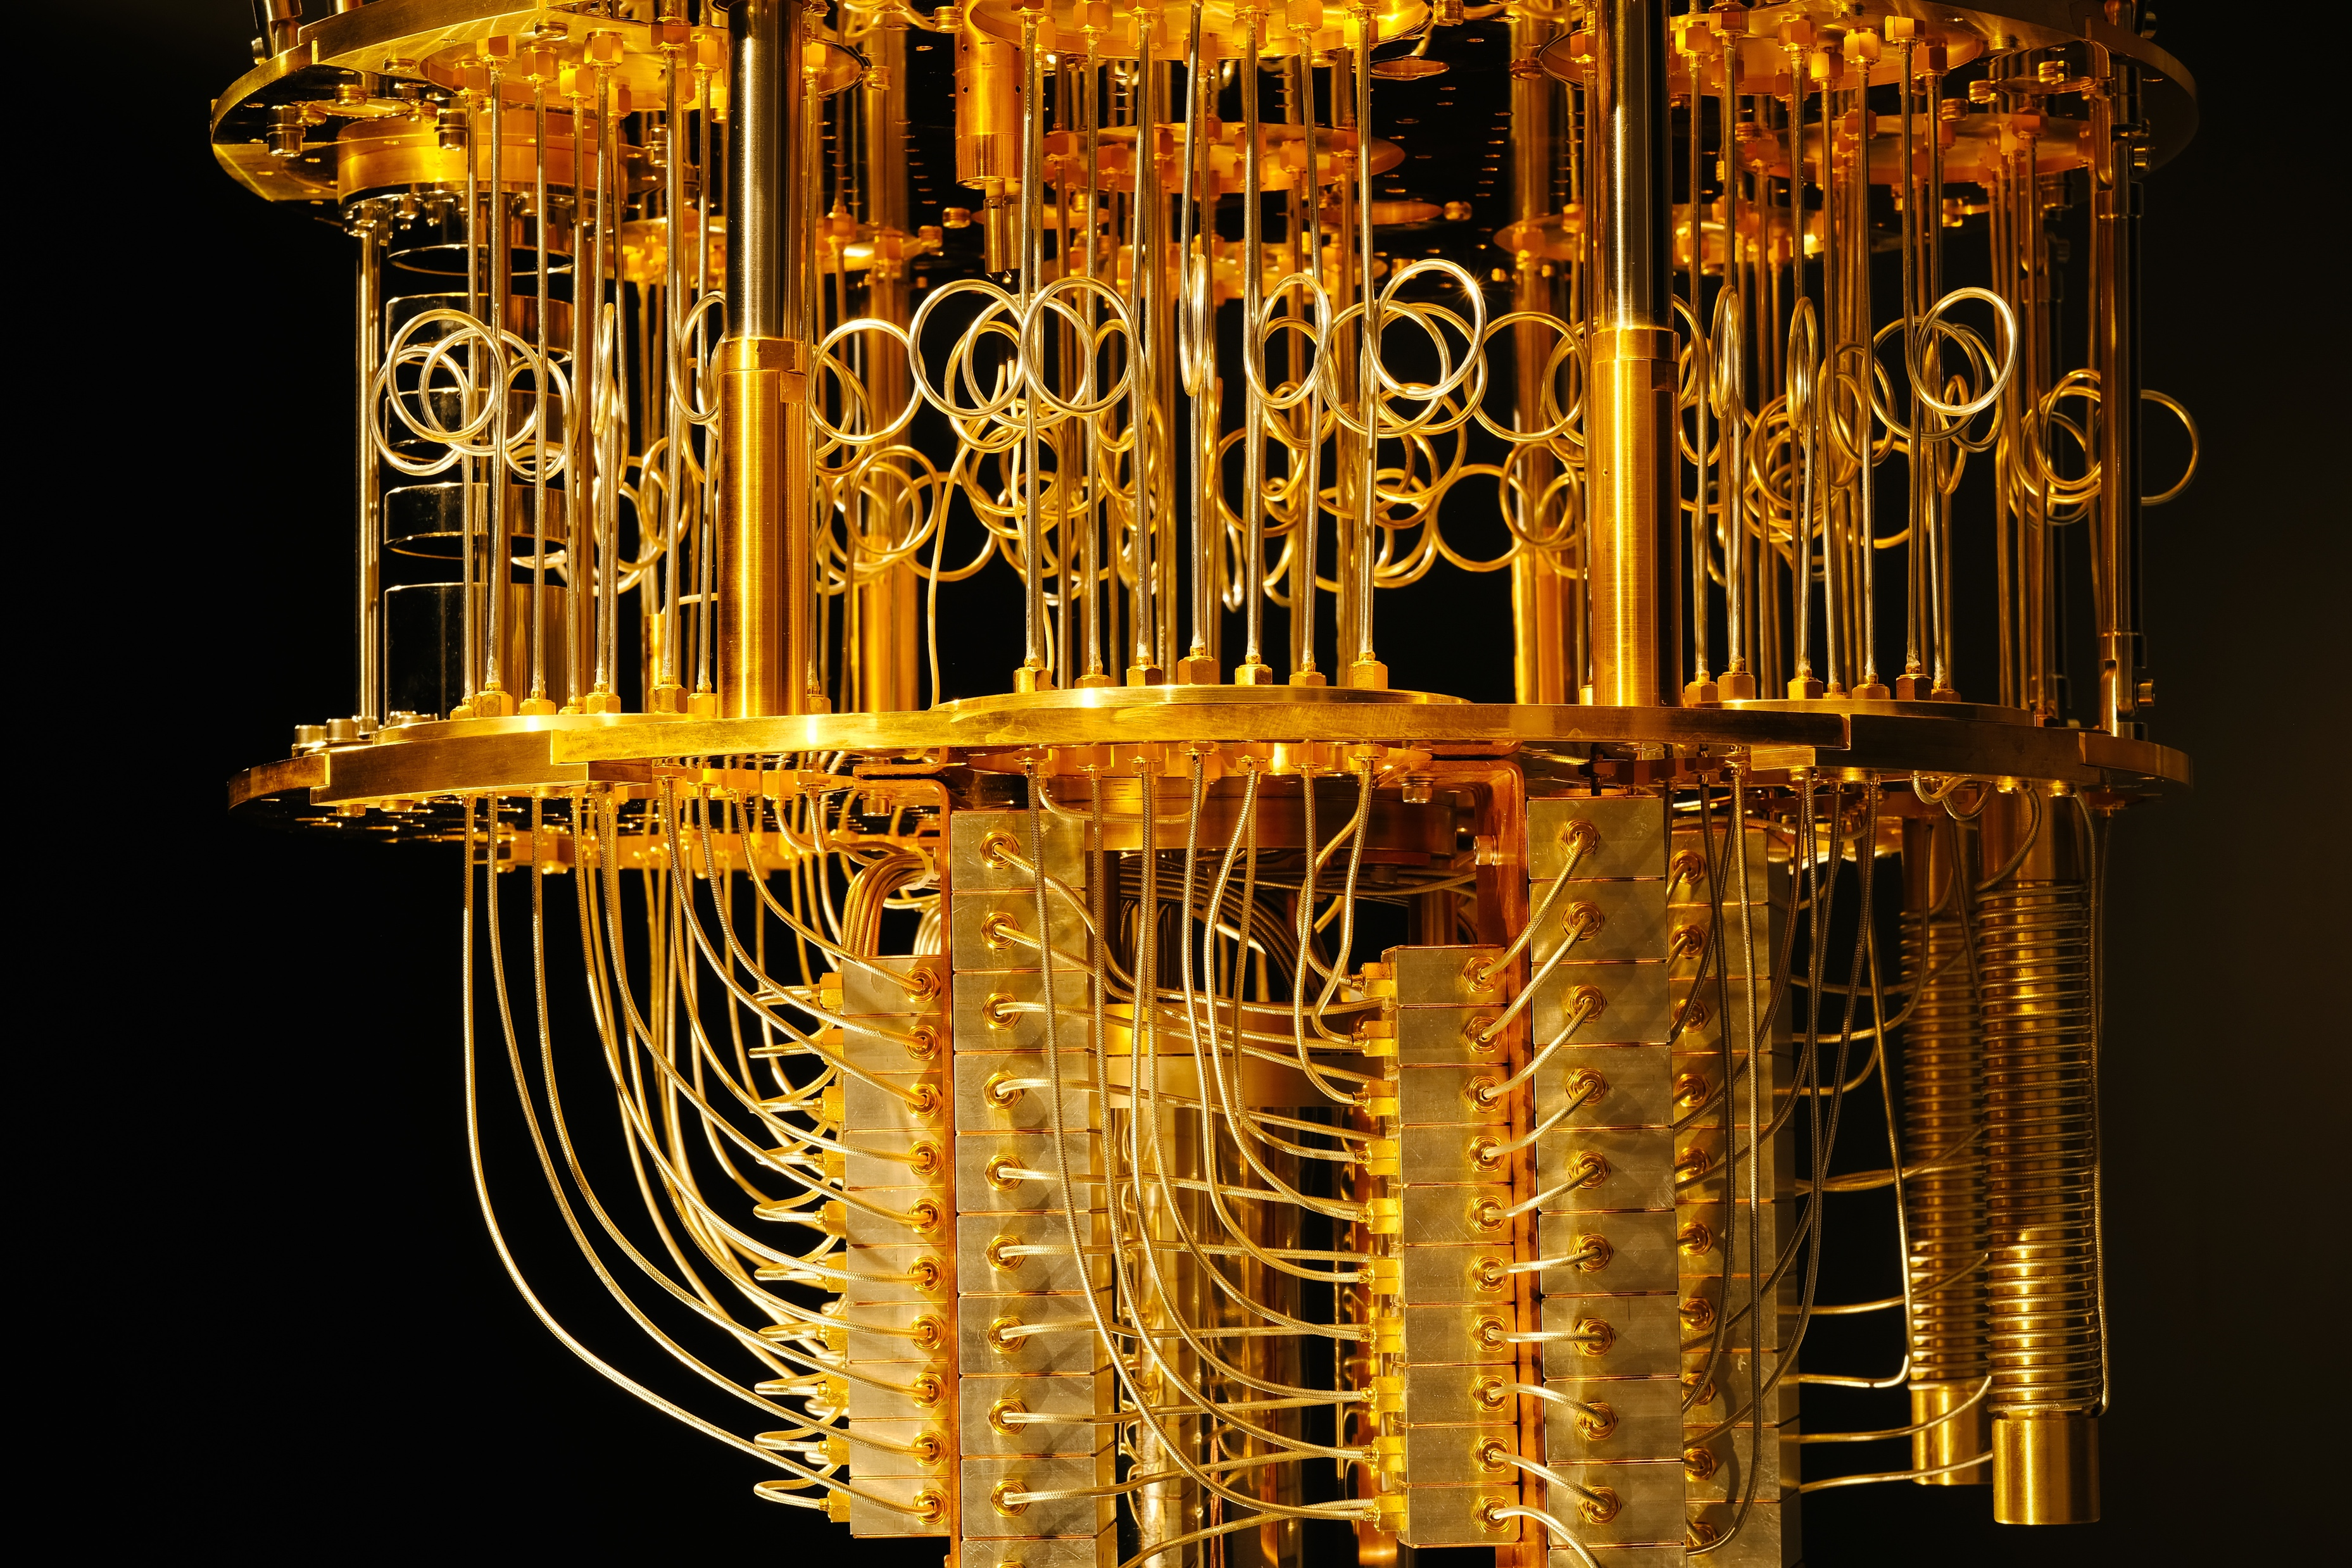
\includegraphics[height=.45\textheight]{fridge.jpg}\\
            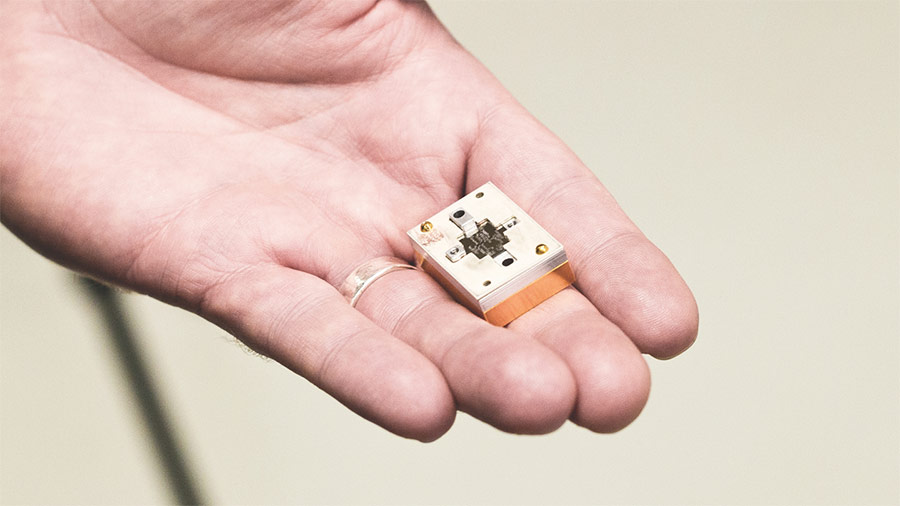
\includegraphics[height=.45\textheight]{inside-4.jpg}
    \end{columns}
\end{frame}

\begin{frame}
    \frametitle{Quantum Chips}
    \begin{columns}
        \column{.45\linewidth}
            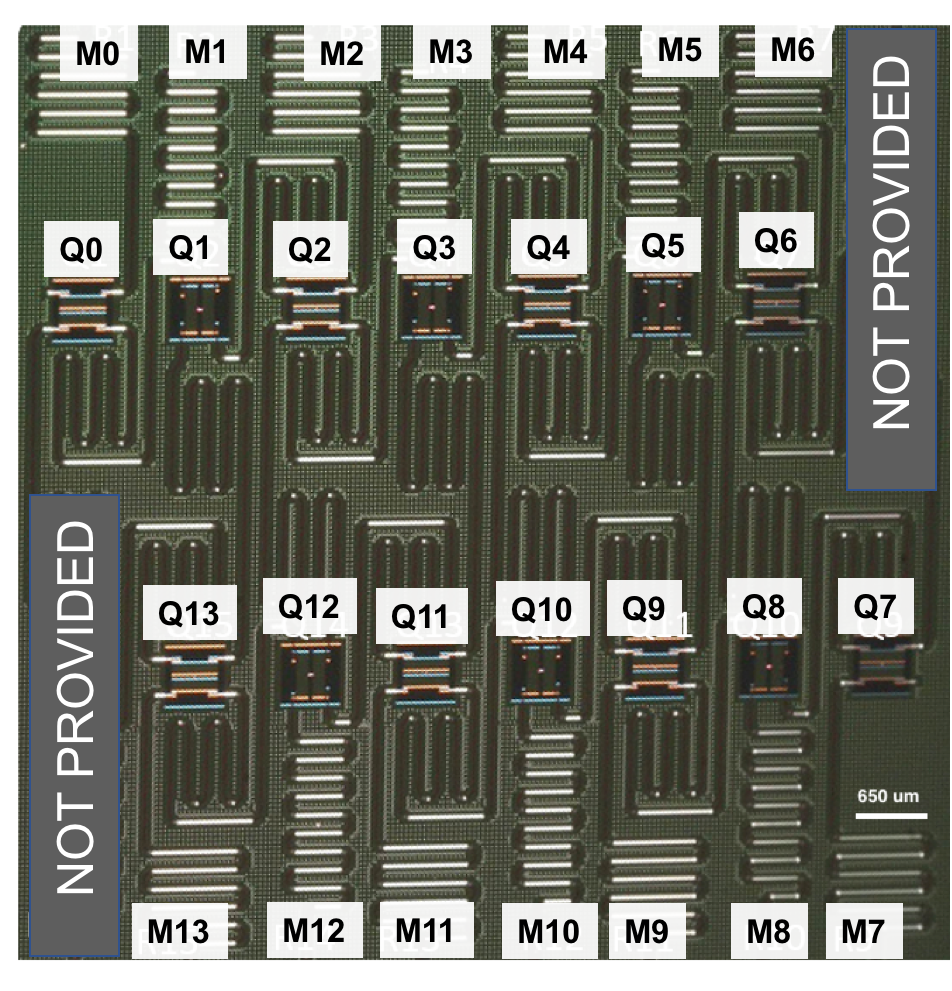
\includegraphics[width=\textwidth]{melbourne-labeled.png}
        \column{.45\linewidth}
            \includegraphics[width=\textwidth]{ibmqx4-labeled.png}
    \end{columns}
\end{frame}

\begin{frame}
    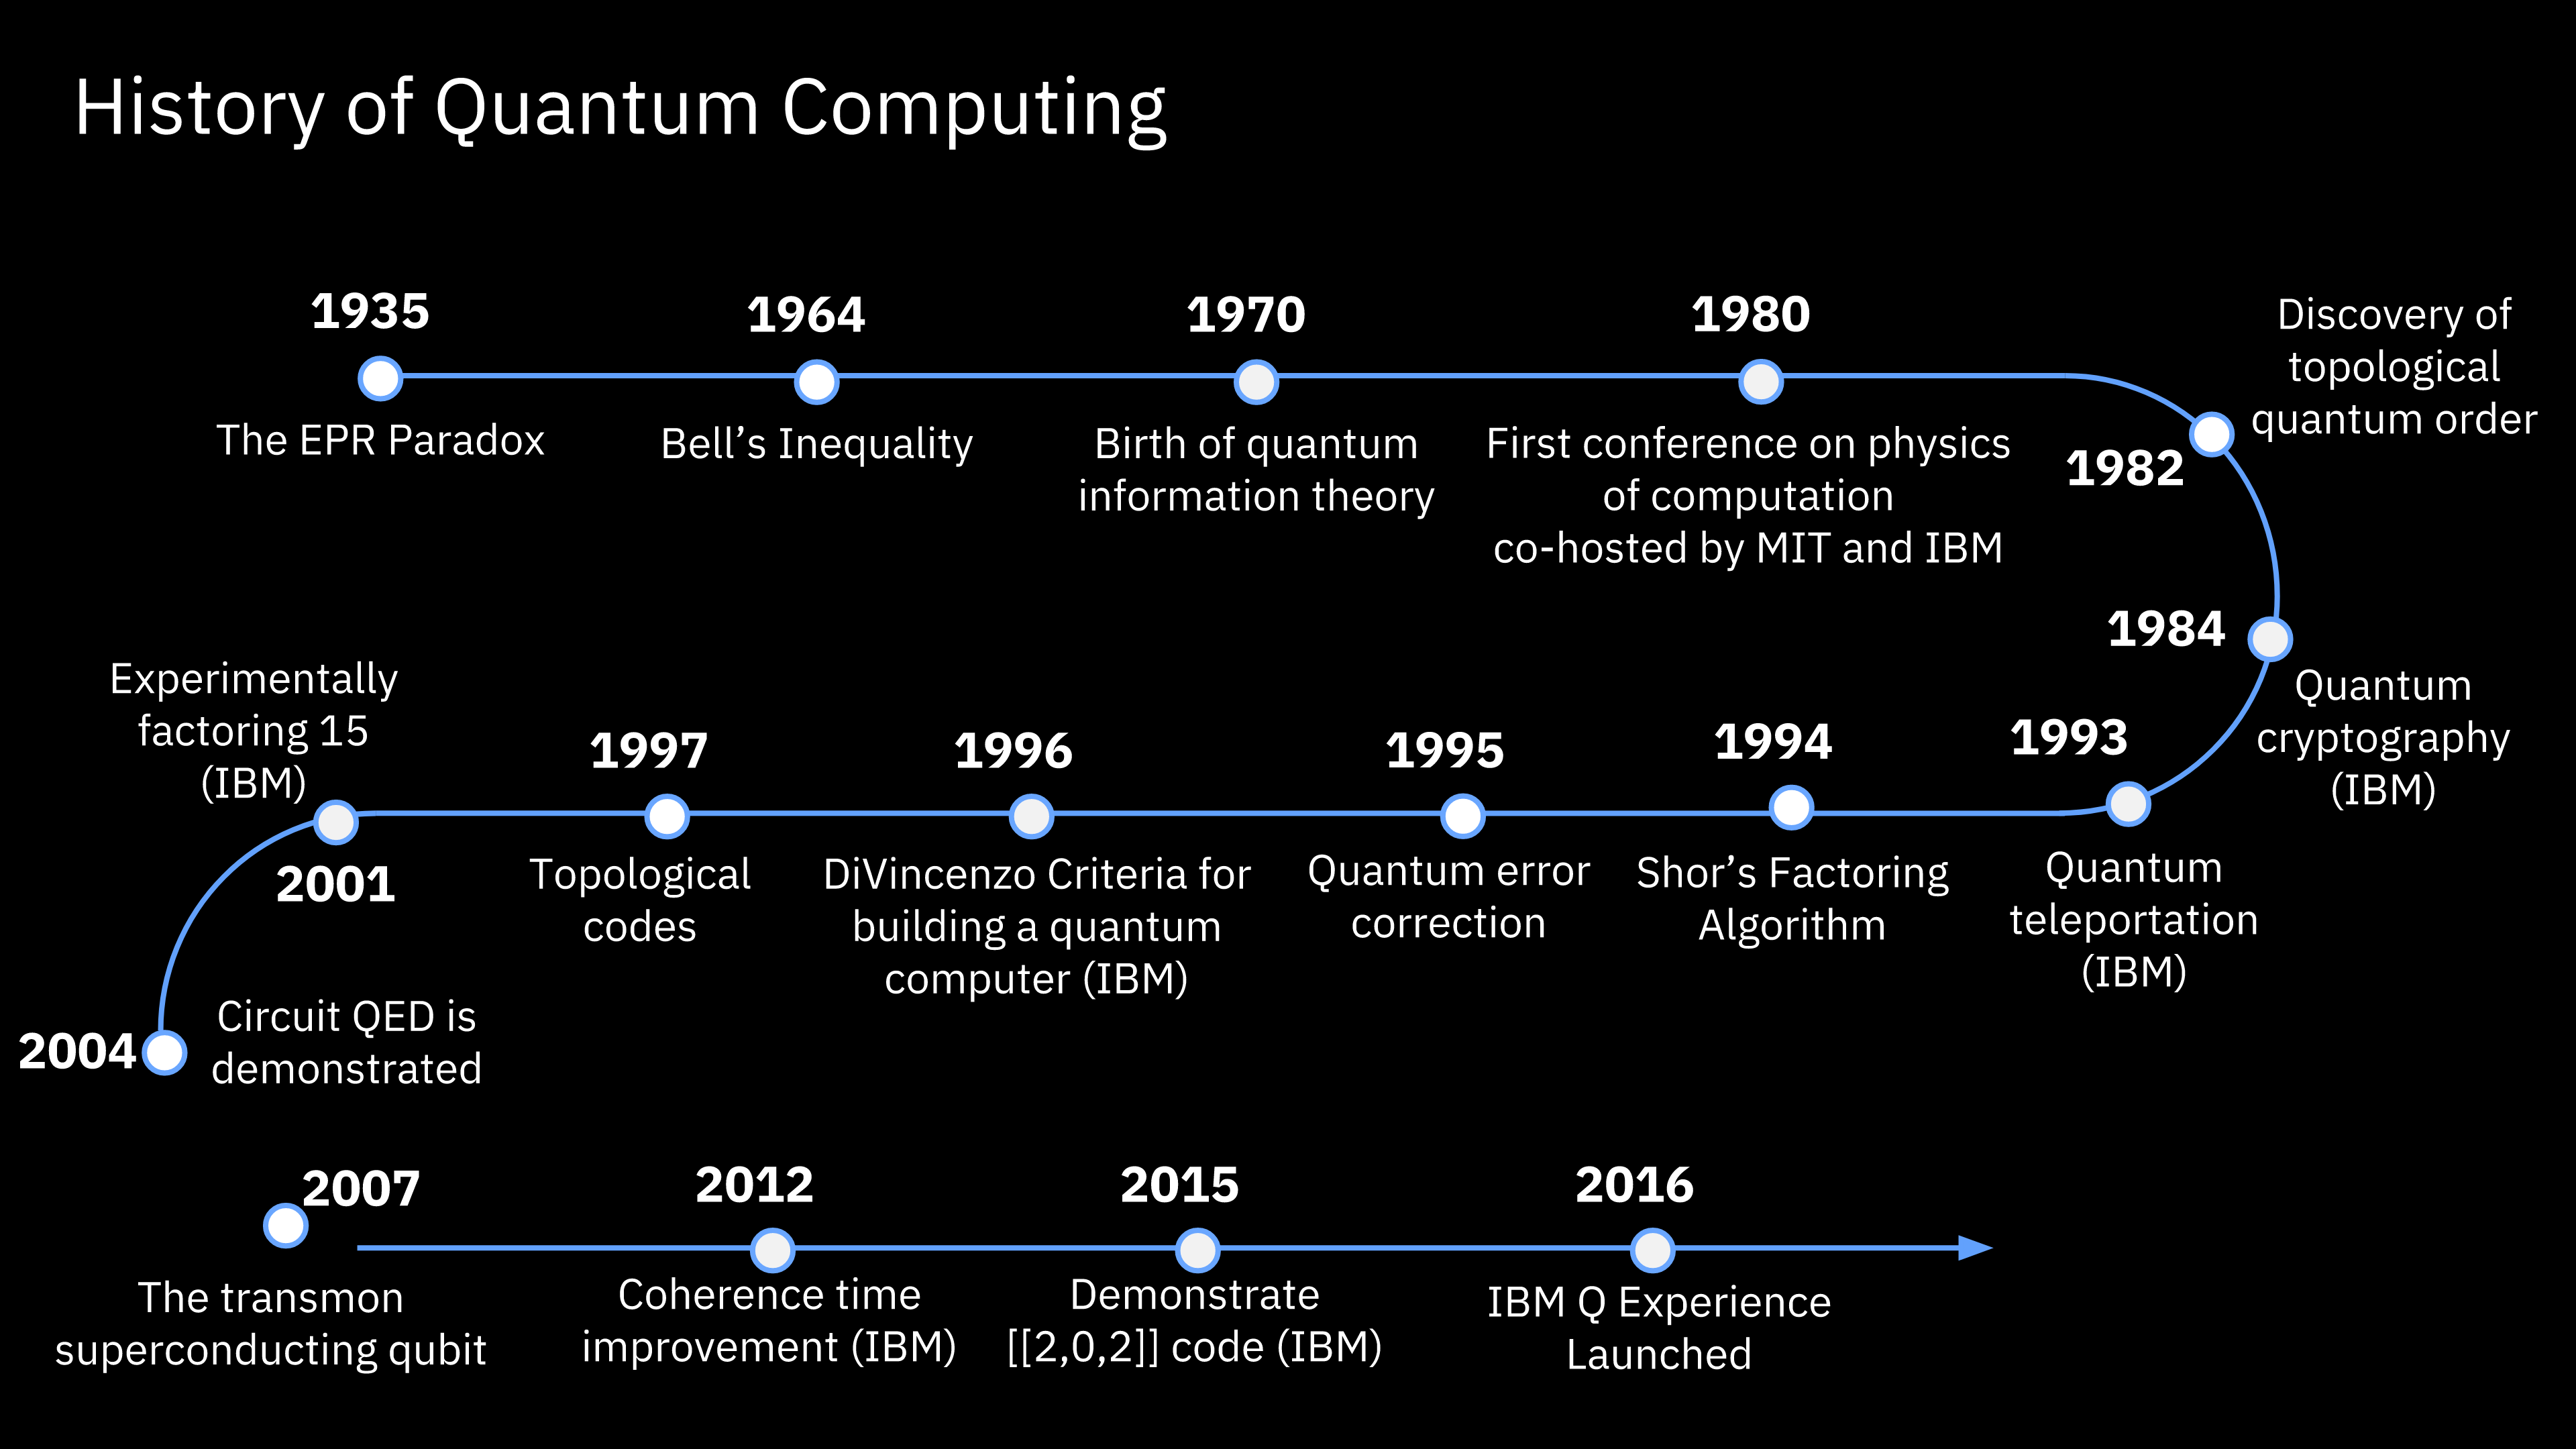
\includegraphics[width=\textwidth]{timeline.png}
\end{frame}


\begin{frame}
    \frametitle{What is Qiskit?}
    \begin{itemize}
        \item Toolkit
    \end{itemize}
\end{frame}

\begin{frame}
    \frametitle{Qiskit}
    \centering
    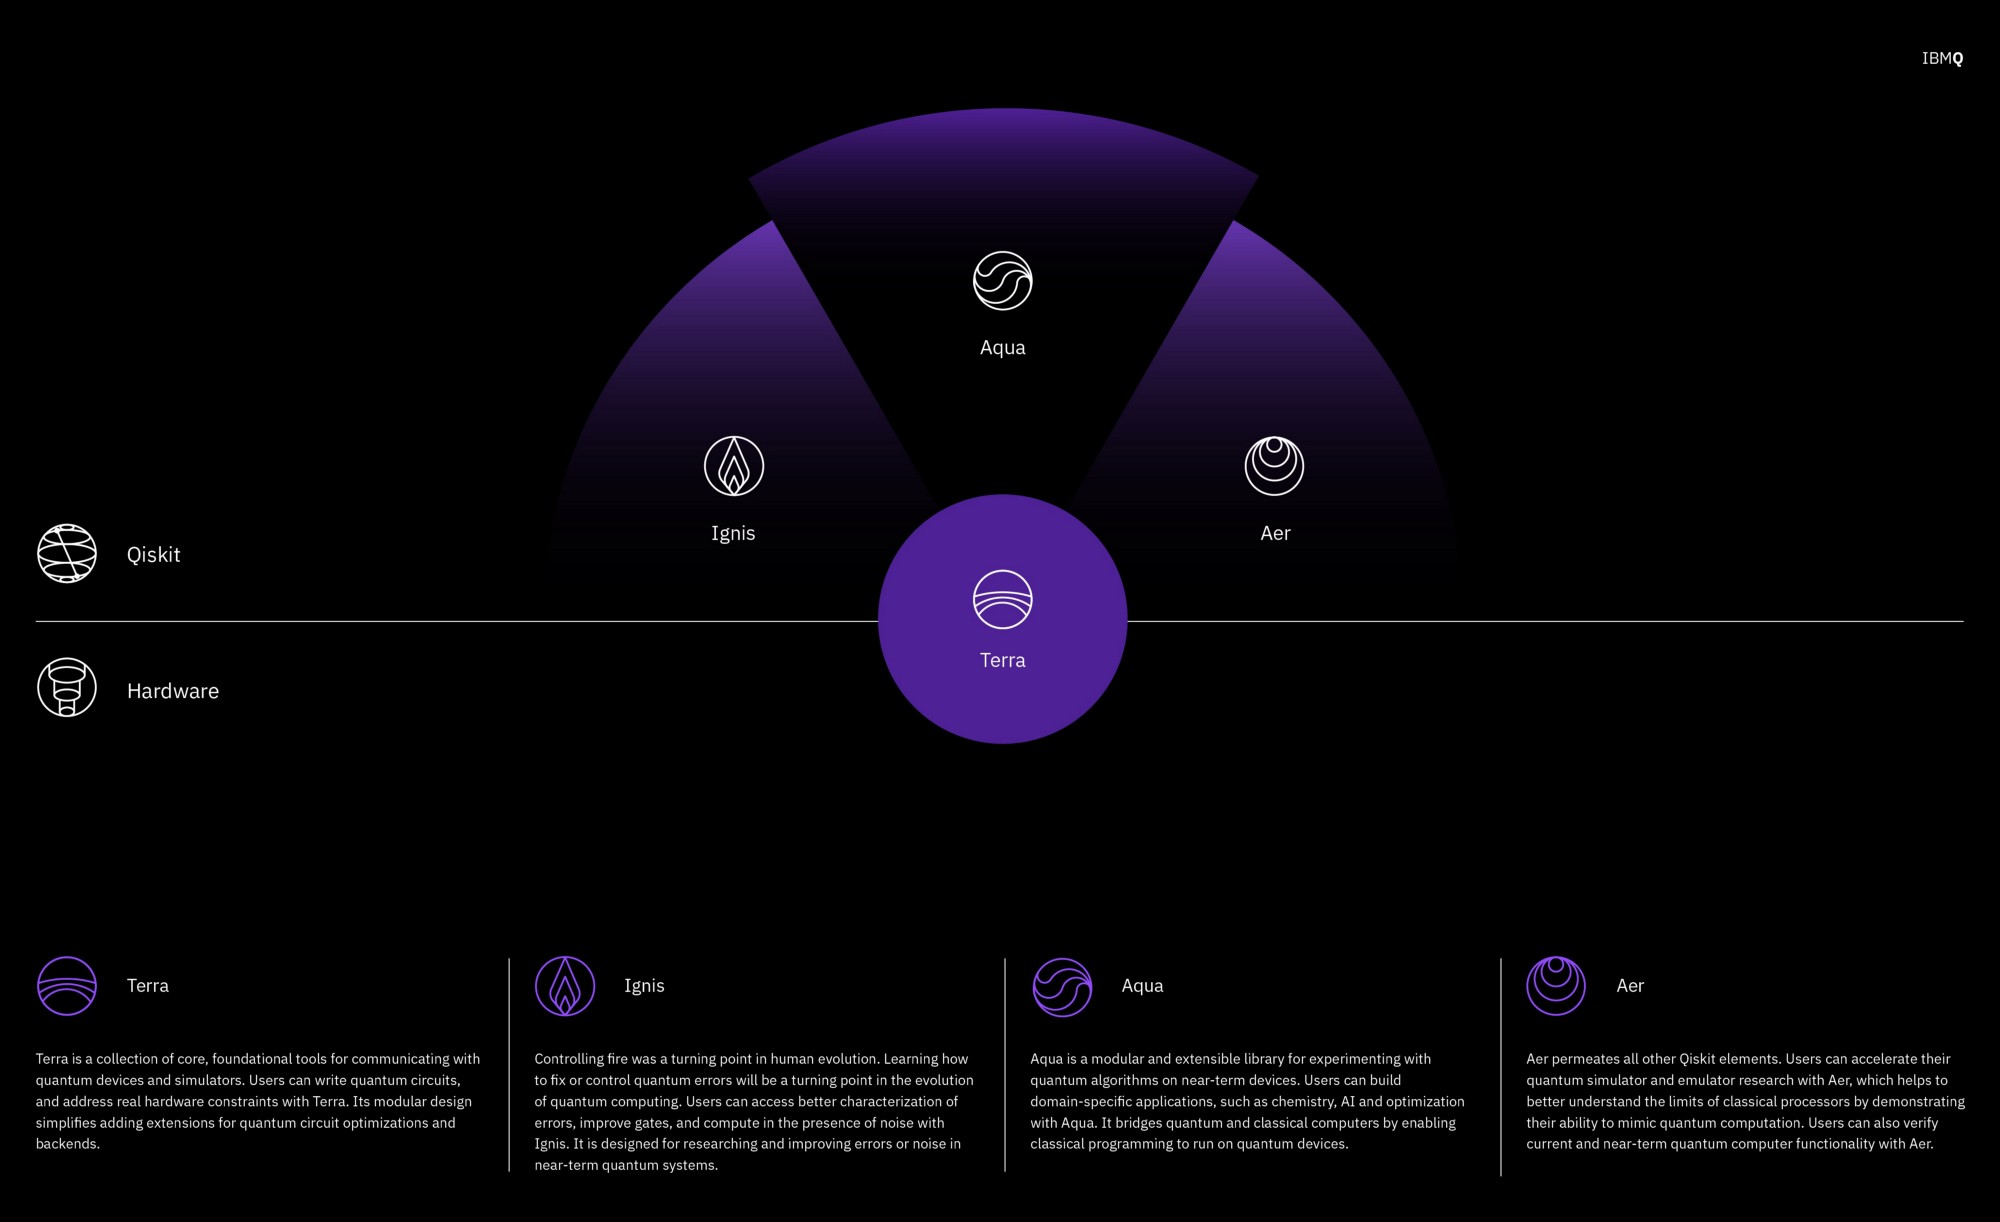
\includegraphics[width=.9\textwidth]{qiskit-components.jpeg}
\end{frame}

\section{Quantum Information Theory}
\begin{frame}
    \frametitle{The Qubit}
    \begin{columns}
        \column{.4\textwidth}
            \begin{itemize}
                \item Bloch
                \item Measure along Z
            \end{itemize}
        \column{.6\textwidth}
            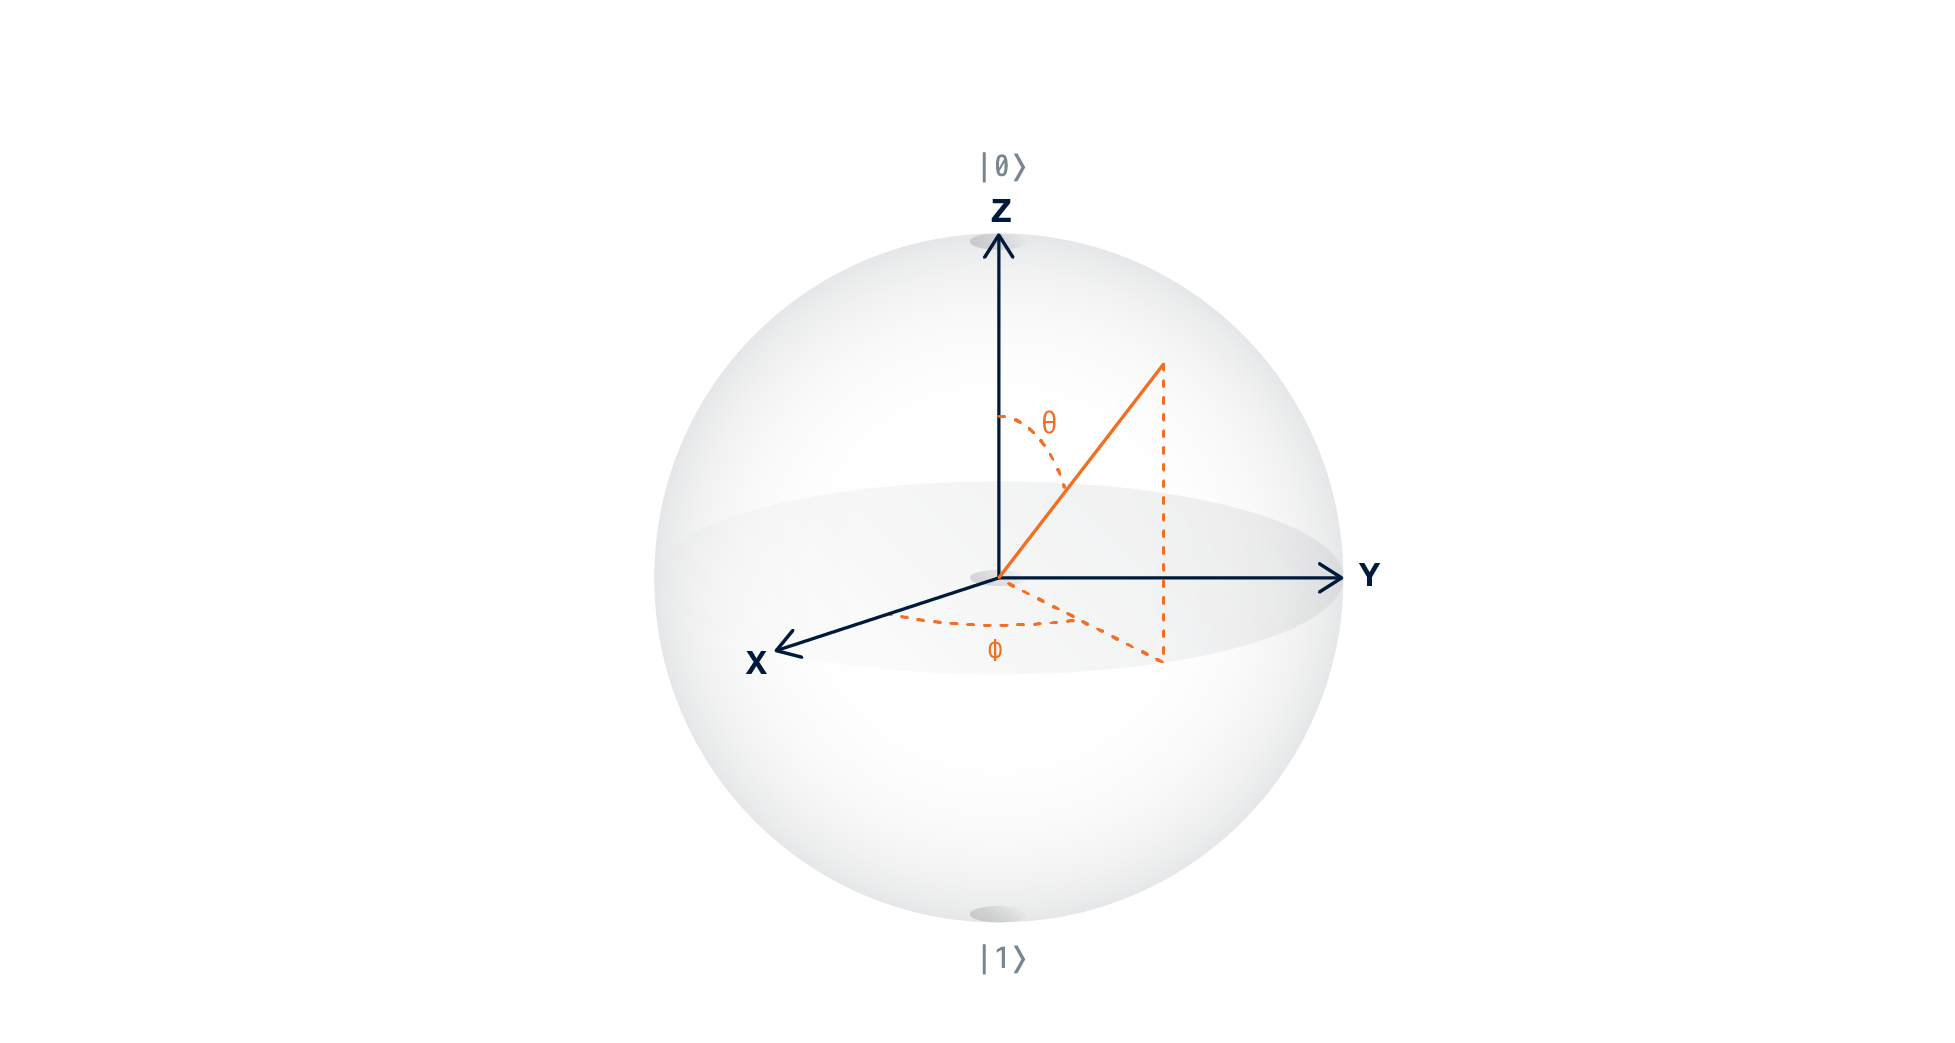
\includegraphics[width=\textwidth]{bloch_angles.png}
    \end{columns}
\end{frame}

\begin{frame}
    \frametitle{Multiple Qubits}

\end{frame}

\subsection{Quantum Gates and Quantum Circuits}
\begin{frame}
    \frametitle{Quantum Gates}
\end{frame}

\begin{frame}
    \begin{columns}[onlytextwidth]
        \begin{column}{.333\textwidth}
            \centering
            \textbf{Gate}
            \begin{equation*}
                \Qcircuit @C=0.5em @R=0.0em @!R {
	 	            \lstick{\ket{0}} & \gate{X} & \qw & \qw\\
            	}
            \end{equation*} \\
            \begin{equation*}
                \Qcircuit @C=0.5em @R=0.0em @!R {
    	         	\lstick{\ket{0}} & \gate{Y} & \qw & \qw\\
    	        }
            \end{equation*} \\
            \begin{equation*}
                \Qcircuit @C=0.5em @R=0.0em @!R {
    	         	\lstick{\ket{0}} & \gate{Z} & \qw & \qw\\
    	        }
            \end{equation*}
        \end{column}
        \begin{column}{.333\textwidth}
            \centering
            \textbf{Matrix Form}
            \[\begin{bmatrix}
                0 & 1\\
                1 & 0 \\
            \end{bmatrix}\]\\
            \[\begin{bmatrix}
                0 & -\iu \\
                \iu & 0 \\
            \end{bmatrix}\] \\
            \[\begin{bmatrix}
                1 & 0 \\
                0 & -1\\
            \end{bmatrix}\]
        \end{column}
        \begin{column}{.333\textwidth}
            \centering
            \textbf{Bloch Sphere}
            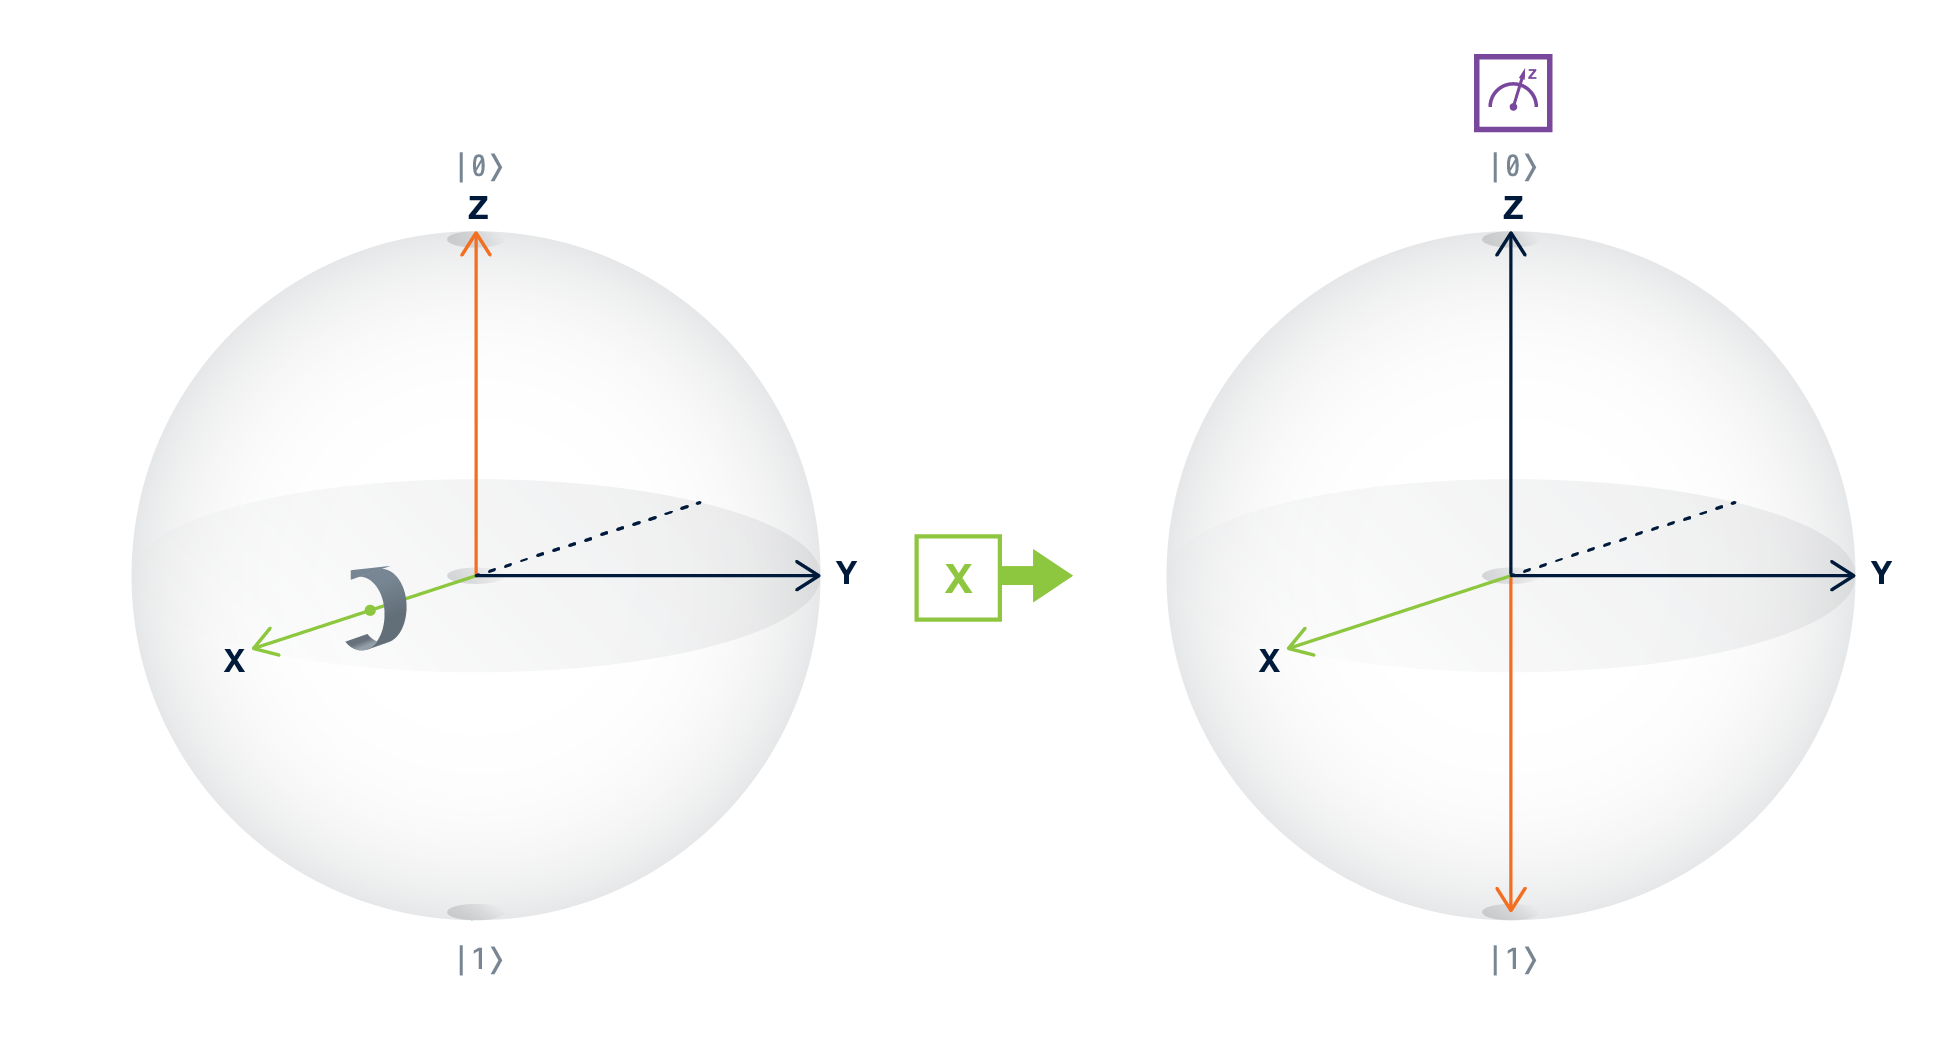
\includegraphics[width=\textwidth]{gate_x_bloch.png}\\
            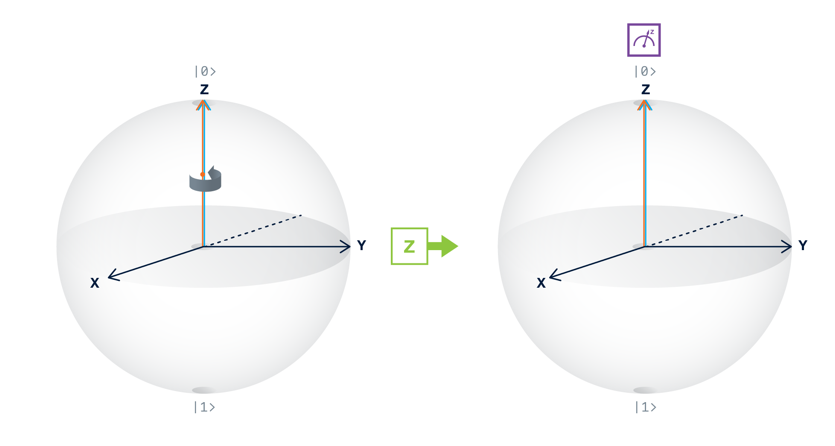
\includegraphics[width=\textwidth]{gate_z_bloch.png}\\
        \end{column}
    \end{columns}
\end{frame}

\begin{frame}
    \frametitle{Superposition and Hadamard Gate}
    \begin{columns}
        \column{.5\textwidth}
        \begin{equation*}
            \Qcircuit @C=0.5em @R=0.0em @!R {
	 	        \lstick{\ket{0}} & \gate{H} & \qw & \qw\\
    	     }
        \end{equation*}
        \column{.5\textwidth}
        \[\frac{1}{\sqrt{2}} \begin{bmatrix}
            1 & 1 \\
            1 & -1 \\
        \end{bmatrix}\]
    \end{columns}
    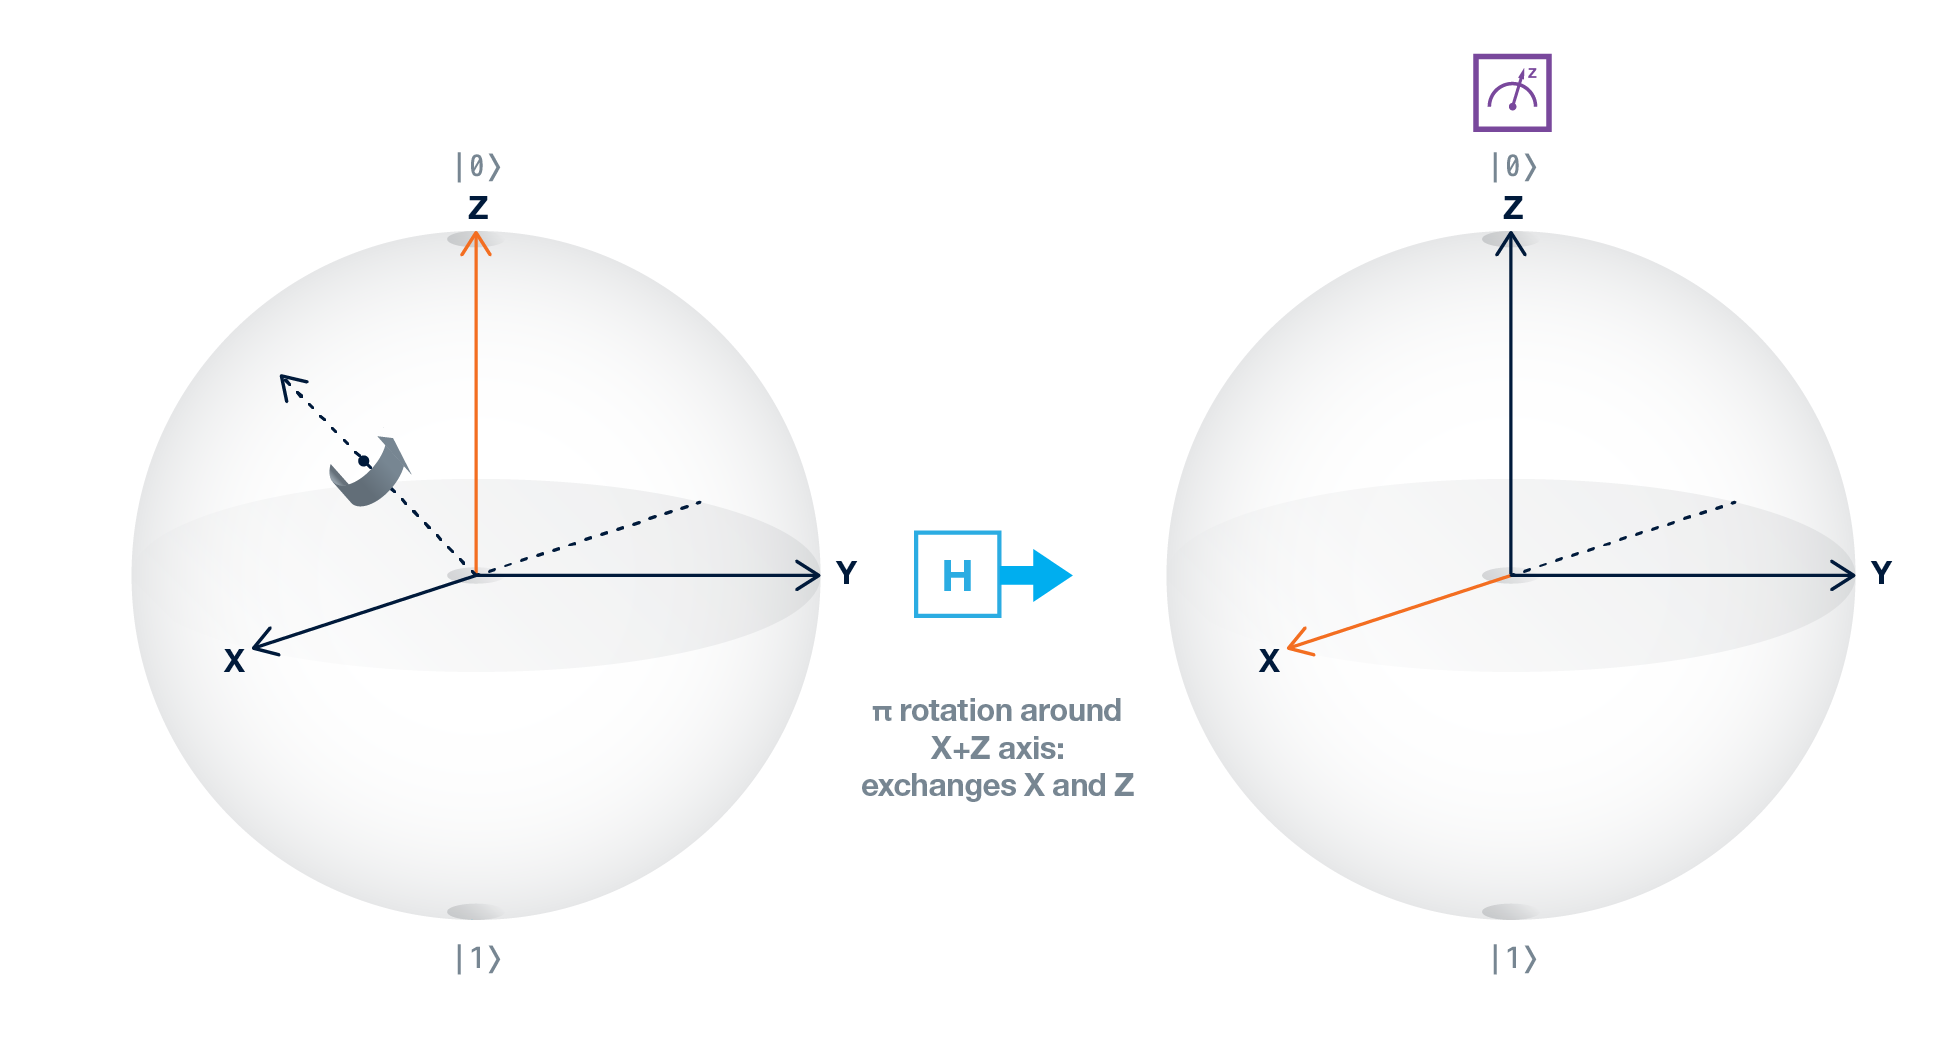
\includegraphics[width=\textwidth]{gate_h_bloch.png}
\end{frame}

\begin{frame}
    \frametitle{Phase}

\end{frame}

\begin{frame}
    \frametitle{Controlled Not Gate}

    \begin{equation*}
        \Qcircuit {
            \lstick{\ket{0}}  & \ctrl{1} & \rstick{\ket{0}} \qw \\ 
            \lstick{a\ket{0} + b\ket{1}} &  \targ & \rstick{a\ket{0} + b\ket{1}} \qw \\
    }
    \end{equation*}

    \begin{equation*}
        \Qcircuit {
            \lstick{\ket{1}} & \ctrl{1} & \rstick{\ket{1}} \qw\\ 
            \lstick{a\ket{0} + b\ket{1}} & \targ & \rstick{b\ket{0} + a\ket{1}} \qw\\
    }
    \end{equation*}
    \centering
    \textbf{CNOT flips the \textit{target} bit if the \textit{control} bit is 1}
\end{frame}

\begin{frame}
    \frametitle{Quantum Circuits}
    \begin{equation*}
        \Qcircuit @C=0.5em @R=0.0em @!R {
        \lstick{q0_{2}: \ket{0}} & \qw & \gate{H} & \ctrl{1} & \gate{X} & \meter & \qw & \qw & \qw & \qw\\
        \lstick{q0_{1}: \ket{0}} & \gate{X} & \gate{H} & \targ & \qw & \qw & \meter & \qw & \qw\\
        \lstick{q0_{0}: \ket{0}} & \qw & \gate{H} & \qw & \qw & \qw & \qw & \meter & \qw & \qw\\
	 	\lstick{c0_{2}: 0} & \cw & \cw & \cw & \cw & \cw \cwx[-3] & \cw & \cw & \cw & \cw\\
	 	\lstick{c0_{1}: 0} & \cw & \cw & \cw & \cw & \cw & \cw \cwx[-3] & \cw & \cw & \cw\\
	 	\lstick{c0_{0}: 0} & \cw & \cw & \cw & \cw & \cw & \cw & \cw \cwx[-3] & \cw & \cw\\
	 }
    \end{equation*}
\end{frame}

\section{Example Application}
\begin{frame}
    \frametitle{Bernstein-Vazirani Algorithm\footnotemark}
    \begin{columns}
        \column{.3\textwidth}
            \centering
            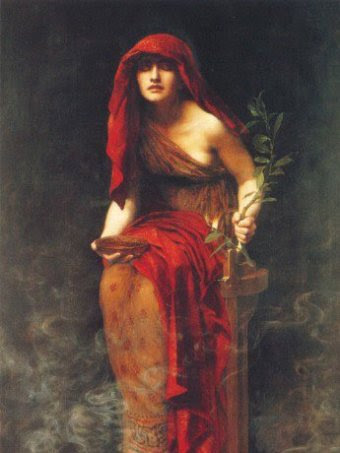
\includegraphics[width=\textwidth]{the_oracle.jpg} \\
            \large \textbf{The Oracle}
        \column{.7\textwidth}
        Input (query)\\
        $\Longleftarrow X_{n-1} \dotsb \ X_{1} X_{0} $\\
        \vspace{1.5em}
        Secret Bitstring\\
        $ \boxed{S_{n-1} \dotsb S_{1} S_{0}} $\\
        \vspace{1.5em} 
        Output (result)\\ 
		$\Longrightarrow X_{n-1}S_{n-1} \oplus \dotsb X_{1}S_{1} \oplus X_{0}S_{0} $\\
    \end{columns}
    \vspace{3em}
    \footnotetext[1]{E. Bernstein \& U. Vazirani, STOC, 93}
\end{frame}

\begin{frame}
    \frametitle{Classical Oracle}
	\begin{columns}
		\column{.3\textwidth}
              \centering
              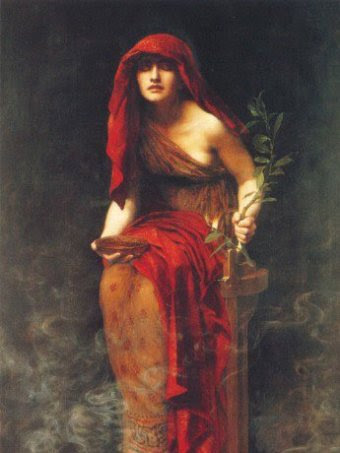
\includegraphics[width=\textwidth]{the_oracle.jpg}
		\column{.7\textwidth}
			O(n)
	\end{columns}
\end{frame}

\begin{frame}
    \frametitle{Quantum Oracle}
	\begin{columns}   
          \column{.3\textwidth}
                \centering
                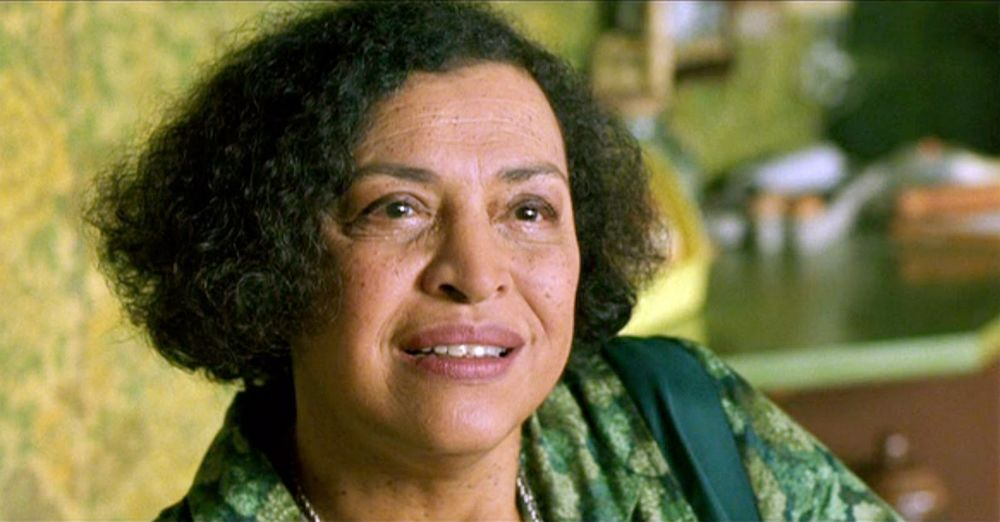
\includegraphics[width=\textwidth]{quantum_oracle.jpg}
          \column{.7\textwidth}
			$O(1)$
	\end{columns}
\end{frame}

\begin{frame}
    \frametitle{Phase Kickback}

\end{frame}

\begin{frame}
    \frametitle{Implementing a Quantum Oracle}

\end{frame}

\begin{frame}
    \frametitle{Live Demo}
\end{frame}


\section{Conclusion}
\subsection{Other Open Source Tools}
\begin{frame}
    \frametitle{Open Source in Quantum Computing}

\end{frame}

\begin{frame}
    \frametitle{Other Open Source Tools}
    \begin{itemize}
        \item https://github.com/rigetticomputing/pyquil
        \item https://github.com/ProjectQ-Framework/ProjectQ
        \item https://github.com/quantumlib/Cirq
        \item https://github.com/qutip/qutip
        \item https://github.com/XanaduAI/strawberryfields
    \end{itemize}
    A lot more out there:
    https://github.com/topics/quantum-computing
\end{frame}

\begin{frame}
    \frametitle{Conclusions}
    \begin{itemize}
        \item Quantum Computing is about solving problems that we can't with
            classical computers
        \item It's not just in labs anymore, quantum computing is accessible by
            everyone now
        \item It's still very early for quantum computers
        \item Open source software is playing a key role early on
    \end{itemize}
\end{frame}

\section{Questions?}
\begin{frame}
\frametitle{Where to get more information}
    \begin{itemize}
        \item Overview and Comparison of Gate Level Quantum Software Platforms: \href{https://arxiv.org/abs/1807.02500}{https://arxiv.org/abs/1807.02500}
        \item Qiskit: \href{https://qiskit.org/}{https://qiskit.org/}
        \item IBM Q Experience: \href{https://quantumexperience.ng.bluemix.net/qx}{https://quantumexperience.ng.bluemix.net/qx}
        \item Tutorials on Quantum Computing and Qiskit: \href{https://github.com/Qiskit/qiskit-tutorials}{https://github.com/Qiskit/qiskit-tutorials}
    \end{itemize}
\end{frame}

\end{document}
